\chapter{Implementierung - Pathcompare}
\label{sec:implementierung}
\section{Technischer Rahmen}

\subsection{Robot Operating System - ROS}

Innerhalb des Referenzsystems wird ROS im Zusammenhang mit der Steuerung
des Roboters genutzt und um die während einer Testfahrt gewonnenen Pfaddaten
zu übermitteln. Im Folgenden wird genauer auf die Fähigkeiten und
Ziele von ROS eingegangen.

Obwohl der Name zunächst anderes vermuten lässt, ist ROS kein
Betriebssystem im klassischem Sinne. Es ist vielmehr eine Sammlung von
Anwendungen, welche auf ein Betriebssystem angewiesen sind, um ausgeführt werden
zu können. ROS bietet aber Funktionalitäten, die abstrahiert betrachtet
Betriebssystemfunktionen ähneln. Charakteristisch ist hierbei ROS's Fähigkeit
lokal oder nichtlokal ausgeführte Programme miteinander zu verbinden und eine
strukturierte Kommunikation zwischen diesen zu ermöglichen. Die grundlegenden
Ansätze von ROS sind:

\begin{itemize}
  \item multi-tool Ansatz
  \item verteiltes Rechnen 
  \item peer-to-peer Kommunikation
  \item keine feste Bindung an eine Programmiersprache
  \item frei und Open-Source
\end{itemize}

Multi-tool Ansatz bedeutet, dass ROS die Fähigkeiten verschiedener Programme
und Libraries zur Verfügung stellt. Diese sind jedoch nicht fest in den Kern
von ROS eingebaut, sondern modular integriert. Als analoges Beispiel in
Hinblick auf Betriebssysteme kann man ROS diesbezüglich mit einen Mikrokernel
vergleichen. Die Modularität bietet den Vorteil, dass der ROS Kern
vergleichsweise klein ist. Außerdem müssen während der Ausführung nur wirklich
gebrauchte Tools geladen werden.

Die peer-to-peer Kommunikation bezieht
sich auf die Kommunikation zwischen den ROS Modulen, welche
durch den ROS Kern gesteuert wird. Der Kern von ROS ist ursprünglich in C++
implementiert. Es existieren jedoch bereits Portierungen in andere Sprachen wie
Python, Octave und Lisp, um die ROS-\gls{API} einer größeren Zahl von
Entwicklern und Projekten zur Verfügung zu stellen. 

%TODO hier Referenz zu ROS paper bringen oder später?

ROS ist darüber hinaus frei verfügbar und Open-Source. 
\footnote{\url{www.ros.org/wiki/ROS/Installation}}


Man kann beliebige Programme als Module zur Erweiterung von ROS hinzufügen, wie
es auch im Rahmen des Referenzsystems geschehen ist. Bei allgemeinem Nutzen und
gegebener Pflege der Software besteht die Möglichkeit, dass diese offiziell zu
ROS hinzugefügt werden.

Um die konkreten Abläufe und Komponenten innerhalb von ROS
veranschaulichen zu können und damit auch den Bezug zu Pathcompare herstellen
zu können, ist es zunächst erforderlich die Begrifflichkeiten innerhalb von
ROS zu klären. Im Folgendem werden diese aufgezeigt, siehe dazu auch
\autoref{fig:roscomponents}.

\begin{figure}[t]
  \begin{center}
    \fbox{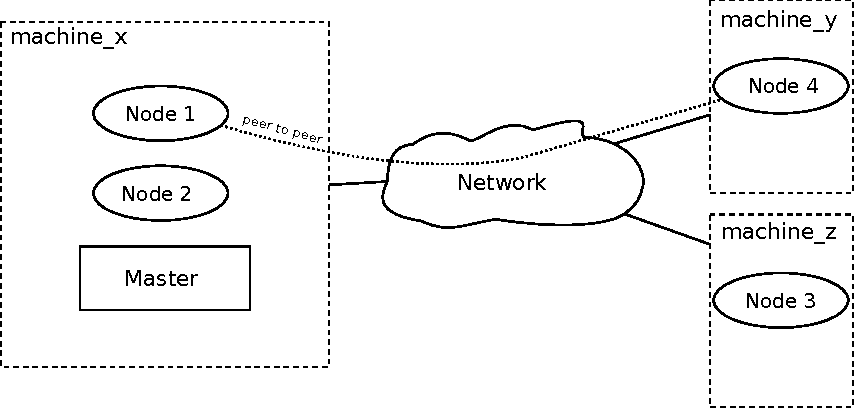
\includegraphics{./graphics/ros_components}}
  \end{center}
  \caption{Beispielhafte Ausführung von ROS auf unterschiedlichen Rechnern}
  \label{fig:roscomponents}
\end{figure}

Im Zentrum von ROS steht der sogenannte \textit{Master}. Dieser wird als
einzelne Instanz gestartet und wartet dann darauf, dass sich Tools, die im
Kontext von ROS gestartet werden, bei ihm anmelden. Ein als Prozess gestartetes
tool wird dabei innerhalb von ROS als \textit{Node} bezeichnet. Ist der
Master nicht gestartet, können auch keine Nodes ausgeführt 
werden. Die Nodes sind also alle zunächst auf Kommunikation mit dem
Master angewiesen. Diese Kommunikation kann lokal oder nichtlokal
ausgeführt werden, d.h. der Master kann sich auch auf einem anderen
Rechner als der Node befinden, solange eine http Verbindung zwischen
beiden hergestellt werden kann. Das Anmelden des Nodes beim
Master erfolgt über einen \gls{XML-RPC} über http. Für den 
Softwareentwickler auf Anwendungsebene ist diese Kommunikation zur Anmeldung
allerdings
vollständig durch die ROS API gekapselt und er muss sich in dieser Hinsicht
nicht explizit um Verbindungsaufbau oder Nachrichtenaustausch kümmern. Wie in
der \autoref{fig:roscomponents} dargestellt, können auch die einzelnen Nodes
auf unterschiedlichen Rechnern ausgeführt werden. Diese zentrale
Fähigkeit von ROS lässt sich beispielsweise vorteilhaft ausnutzen durch:

\begin{itemize}
  \item Verteilung oder Auslagerung rechenintensiver Nodes auf potente Hardware
  \item Zusammenführenung von an unterschiedlichen Stellen gewonnenen Daten.
\end{itemize}

So muss beispielsweise ein mobiler Roboter Bilderkennungsaufgaben nicht selbst
ausführen, sondern kann diese an einen Node weiterleiten der auf einem
Rechencluster ausgeführt wird. Der zweite Punkt, also das Zusammenführen von
Daten ist besonders im Bezug auf diese Arbeit wichtig, da Pfaddaten des
Roboters und der zu testenden Sensorknoten für Pathcompare verfügbar
gemacht werden müssen. Die Kommunikation zwischen Nodeserfolgt über
sogenannte \textit{Messages}. Diese enthalten die serialisierte Form der zu
übertragenden Daten. ROS bietet in seinen Kernpaketen bereits zahlreiche
Definitionen für unterschiedliche Message Typen, aber es ist auch
möglich eigene zu generieren. Dies wird von zahlreichen Paketen getan, um
Daten maßgeschneidert übertragen zu können. Einmal definierte Message
Typen können wiederum rekursiv in anderen Message Typen eingebettet 
werden. Ein Beispiel für eine Message ist in \autoref{lst:transform}
dargestellt. Dieser Message Typ ist standardmäßig in ROS definiert.
Sie besteht wie erkennbar aus den zwei Typen \textit{Vector3} und
\textit{Quaternion}. Letzterer beschreibt die Rotation und Vector3 die
Translation. Zusammengefügt ergibt dies eine Transformationsnachricht.

\begin{lstlisting}[caption=ROS transformation Message, label=lst:transform]
geometry_msgs/Vector3 translation
  float64 x
  float64 y
  float64 z
geometry_msgs/Quaternion rotation
  float64 x
  float64 y
  float64 z
  float64 w
\end{lstlisting}

Soll ein Node seine Messages anderen Nodes senden
können, so muss er dies zunächst durch festlegen einer sogenannten
\textit{Topic} beim Master anmelden. Über den Master wird
dadurch diese Topic für andere Nodes im ROS sichtbar. Eine
Topic ist definiert durch eine sogenannte Topic-id, einem
eindeutigen String. Dieser ist vergleichbar mit einer URL und dient zur
Identifikation innerhalb des ROS. Eine weitere festgelegte
Eigenschaft einer Topic ist der Typ der über sie versendeten
Messages. Nodes welche Messages einer
Topic empfangen sollen, müssen diese Topic dann beim
Master abonnieren. Der Master vermittelt dann eine
peer-to-peer Verbindung zwischen dem Anbieter Node der Topic und dem
Abonnenten. Generell gilt dabei, dass Topics einen unidirektionalen
Kommunikationsweg darstellen. Nur der Anbieter versendet Messages.
Der oder die Abonnenten der Topic sind reine Empfänger. 
In programmatischer Hinsicht wird beim Empfang neuer Nachrichten innerhalb des
Nodes eine festgelegte \textit{callback} Methode aufgerufen, um die
Messages zu bearbeiten. Treffen dabei Messages mit einer höheren
Frequenz ein als abgearbeitet werden können, so kommt es irgendwann zu
Verlusten, wenn die Größe der Message Queue beim Empfänger überschritten
wird. Die Größe der Queue kann jedoch durch die ROS API gesteuert werden.  

Zwei weitere wichtige Begriffe in ROS betreffen die Organisierung der
Dateien, die zu den einzelnen Tools gehören. Dies sind im einzelnen:

\begin{itemize}
  \item Package
  \item Stack
\end{itemize}

Ein \textit{Package} beinhaltet den Code, Libraries sowie die ausführbare Datei
eines Tools bzw. Nodes. In ROS sind für Packages bestimmte
Ordnerstrukturen und Dateien festgelegt, sodass mithilfe der von ROS
mitgebrachten Tools Packages leicht gebaut, gesucht und gestartet
werden können. Beispielsweise basiert das ROS build System auf cmake und so ist
eine vorkonfigurierte cmake Buildatei, genannt \textit{CMakeLists.txt}, in jedem
Package grundsätzlich enthalten. Eine Zusammenfassung mehrerer
Packages wird als \textit{Stack} bezeichnet. 

Überträgt man die vorgestellten ROS Begriffe auf Pathcompare so ist
dieses tool, während der Ausführung,
ein einzelner Node, welcher Topics abonnieren kann, um
Messages zu empfangen. Es wird im Teil Implementierung darauf
eingegangen, welche Messages das genau sind. Alle zum Kompilieren und
Ausführen nötige Dateien sind dabei in zwei Packages namens
\textit{pathcompare} und \textit{pathcompareplugins} aufgeteilt.

\subsection{Qt}

Pathcompare ist darauf ausgelegt alle Informationen für den Nutzer in einer
Benutzeroberfläche ,fortan als GUI bezeichnet, zu visualisieren.  Da die
Anbindung an ROS über C++ erfolgt, lag es nahe, auch die GUI in C++ umzusetzen.
Dazu wurde das Qt Framework gewählt. Qt ist in C++ implementiert, wobei
allerdings auch Anbindungen für zahlreiche andere Sprachen wie z.B.  Java, C\#,
Ruby oder Python existieren. Qt wird seit 1996
\footnote{\url{http://qt.nokia.com/about/who-we-are}} durch Trolltech
veröffentlicht und ist zum Zeitpunkt des Schreibens in der Version 4.7.4
verfügbar. Das Framework besteht dabei mittlerweile nicht mehr nur aus reinen
GUI Bibliotheken, sondern stellt auch Netzwerk-, SQL- und andere
Anwendungs-Bibliothken zur Verfügung.

Ein entscheidender Vorteil des Qt Frameworks ist die gebotene große
Plattformunabhängigkeit.  Gleichzeitig wird für alle unterstützten
Betriebssysteme, deren nativer Look\&Feel verwendet. Mit nativem Look\&Feel
ist gemeint, dass das Erscheinungsbild von GUI Elementen der Qt Anwendung
dem Erscheinungsbild von GUI Elementen des Betriebssystems gleicht.  Für die
Entwicklung von Pathcompare waren neben den GUI Bibliotheken 
folgende Konzepte und Funktionen beim Entwickeln von Nutzen: 
\begin{itemize}
  \item Signal-Slot Konzept
  \item Plattformunabhängigkeit
  \item graphischer GUI Designer 
\end{itemize}

Auf einige dieser Punkte und deren Bezug zu Pathcompare wird nun kurz eingegangen.

Das \textit{Signal-Slot} Konzept dient dazu, bestimmte Objektveränderungen
beobachtenden Objekten mitzuteilen.  Es realisiert also das Entwurfsmuster des
\textit{Observer patterns}. Signal-Slot erspart es dem Programmierer
einen Verweis auf das beobachtende Objekt, durch einen registrierenden
Methodenaufruf beim aktualisierenden Objekt, zu hinterlegen.  Das erleichtert
den Entwicklungsprozess, da nicht mehr explizite Methoden zum Registrieren von
Beobachtern definiert werden müssen. Stattdessen emittiert, im Falle einer
mitzuteilenden Aktualisierung, das aktualisierende Objekt ein sogenanntes
Signal, welches durch einen Qt Makro als \textit{Signal} ausgezeichnet ist. Bei
Beobachter Objekten, die auf dieses Signal reagieren sollen, wird dann eine als
\textit{Slot} deklarierte Methode selbständig aufgerufen. Vorausgesetzt die
Objekte wurden durch einen vorhergegangenen Aufruf, einer von Qt
bereitgestellten, statischen connect Methode, verbunden. Wie bereits
angesprochen erhöht dieses Konzept, durch Wegfall der manuellen Implementierung
von Beobachter Registriermethoden die Flexibilität für den Entwickler deutlich.
Allerdings ist der durch Qt gekapselte Code, welcher durch Auflösung der Makros
und Kompilierung entsteht, aufblähend und dadurch langsamer bei der Ausführung
als eine direkte Implementierung mit Beobachter Registriermethoden. Im
Anwendungsbereich von Pathcompare ist diese Verlangsamung aber unmerklich und
wiegt nicht die Vorteile für den Entwickler auf. Deshalb wurde das Konzept auch
bei der Entwicklung von Pathcompare eingesetzt. 

Im Zusammenhang mit dem Signal-Slot Konzepts wurde bereits erwähnt, dass Qt C++
um verschiedenen Makros erweitert. Diese Makros werden dabei nicht immer direkt
in gültigen C++ Code übersetzt, sondern dienen als Annotationen. Dies hat
Folgen für den Build Vorgang, denn die mit Annotationen versehenen Klassen
müssen zuerst mit dem von Qt bereitgestellten \gls{MOC} übersetzt werden.
Durch den MOC wird aus den mit Annotationen versehenem C++ Code, erneut C++
Code erzeugt, der anschließend durch weitere Compiler übersetzt werden kann.
Standardmäßig wird in Qt das Build Programm qmake verwendet, welches
die nötigen Aufrufe des MOC automatisch veranlasst. In Hinblick auf
Pathcompare war aber eine Integration in das von ROS genutzte Build
verfahren cmake notwendig. Hierbei muss beachtet werden, dass cmake die
Dateien, welche einen MOC Aufruf notwendig machen, derzeit nicht
selbständig erkennt. Diese müssen manuell in der Buildkonfigurationsdatei,
genannt \textit{CMakeLists.txt}, deklariert werden.  Eine solche CMakeLists.txt
Datei ist in jedem ROS Package vorhanden und muss für dieses angepasst werden.
Die sonstige Einbindung Qt-spezifischer Libraries und deren Verlinkung
mit der Applikation ist in cmake in wenigen Zeilen deklariert. Somit war
insgesamt die Verwendung von Qt in Pathcompare kein Hindernis für die
Verwendung von cmake. Die Nutzung von cmake wird darüber hinaus, für große
Projekte, von der Qt Dokumentation selbst empfohlen.
\footnote{\url{http://developer.qt.nokia.com/quarterly/view/using_cmake_to_build_qt_projects}}
%TODO Quelle Doku Eintrag anbringen?

Neben dem MOC existiert noch ein sogenannter \gls{UIC}. Dieser tritt im
Zusammenhang mit dem graphischen GUI Designer in Erscheinung. 
Beim Erstellen einer GUI mit dem sogenannten
QtDesigner wird eine XML Datei erstellt, welche den Aufbau der GUI abbildet.
Der UIC ist dann dafür verantwortlich, diese Datei in C++ Klassen zu übersetzen.
Auch hier muss cmake veranlasst werden zunächst für einen UIC Aufruf
entsprechender Dateien zu sorgen.

%TODO Quelle Plug-in Seite anbringen?

\section{Design der Software}
Wie bereits im Abschnitt ``Aufgabenstellung'' erwähnt, lag der Fokus beim
Design der Pathcompare GUI darauf, einfache Benutzung und übersichtliche
Darstellung der Informationen für den Nutzer zu gewährleisten.  Außerdem sollte
die Software leicht erweiterbar sein, um flexibel auf neue Testbedingungen oder
geänderte Anforderungen reagieren zu können. Im folgenden Abschnitt wird
beschrieben wie Pathcompare diese Ziele realisiert.

\subsection{Überblick Gesamtsystem}

Im Folgenden wird die Software in einer Gesamtansicht dargestellt und
anschließend auf die Funktionsweise ihrer Einzelkomponenten genauer eingegangen.

Wie erwähnt ist Pathcompare durch
Plug-ins erweiterbar. Dadurch kann man zunächst das Gesamtsystem in zwei Teile
untergliedern:

\begin{enumerate}
  \item Rahmen
  \item Plug-ins
\end{enumerate}

Rahmen und Plug-ins sind dabei in zwei unterschiedlichen ROS Packages
organisiert. Das Package \textit{pathcompare} beinhaltet alle den Rahmen betreffenden
Dateien und das Package \textit{pathcompareplugins} beinhaltet die Plug-ins.
Die Aufteilung spiegelt sich auch in der GUI wider.
Hierbei bildet die GUI des Rahmens die Grundlage für die Visualisierung von Plug-ins.
Dabei wird den Plug-ins, nachdem sie geladen wurden, ein Platz innerhalb des
Rahmens zugewiesen. Innerhalb dieses zugewiesenen Platzes können sie beliebige
eigene GUI Elemente laden und haben die volle Kontrolle über diese. Insgesamt
gehören die drei in \autoref{fig:pathcompare} abgebildeten GUI Elemente zum
Rahmen, dies sind:

\begin{itemize}
\item Hauptfenster
\item Topic Übersicht
\item Plug-in Tab-Fenster
\end{itemize}

Das Hauptfenster dient dabei als Grundlage für die Topic Übersicht und das
Plug-in Tab-Fenster. Die Topic Übersicht und das Plug-in Tab-Fenster sind vertikal
getrennt. Die Topic Übersicht ist dabei ganz links angeordnet.

\begin{figure}[t]
  \begin{center}
    \fbox{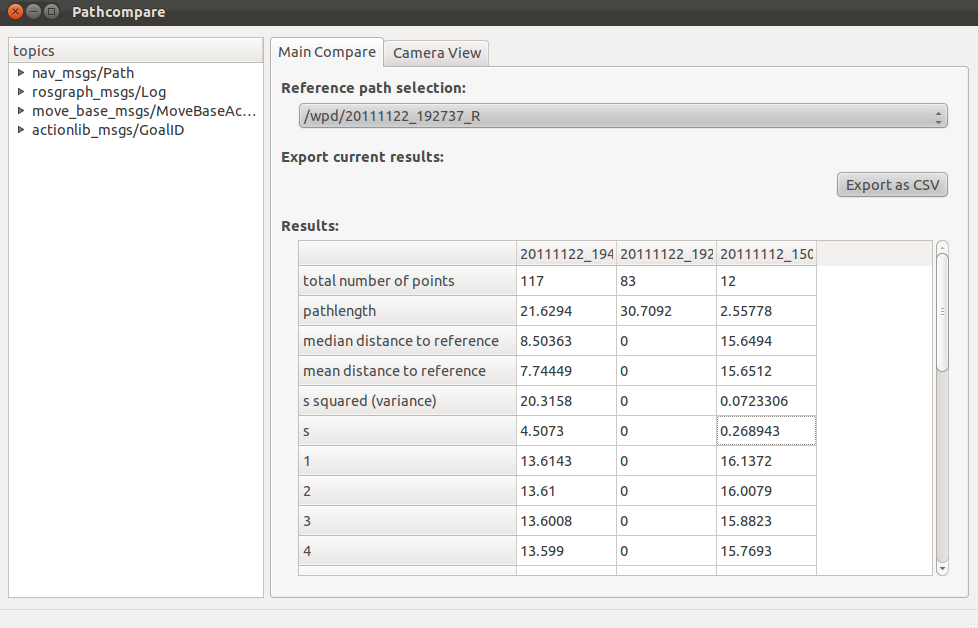
\includegraphics{./graphics/screenshotpathcompare4}}
  \end{center}
  \caption{Hauptansicht von Pathcompare mit geladenen Plug-ins}
  \label{fig:pathcompare}
\end{figure}

Rechts neben der Topic Übersicht schließt unmittelbar das Plug-in Tab-Fenster
an. Wird ein Plug-in geladen, wird in diesem Tab-Fenster ein neuer Tab
angelegt. Die Fläche dieses Tabs wird diesem Plug-in dann zur Verfügung
gestellt um seine GUI darauf aufzubauen. Auf Details bezüglich des Ladens der
Plug-ins und deren Funktionsweise wird im Abschnitt ``Main
Compare Plug-in'' eingegangen. 

Die Topic Übersicht zeigt die momentan im ROS verfügbaren Topics an.  Um die
Topic Übersicht zu strukturieren sind Topics desselben Message Typs in Gruppen
zusammengefasst dargestellt.  Diese Gruppen werden dann kompakt im Topic
Übersicht Fenster angezeigt und können dort durch den Nutzer aufgeklappt
werden, um alle Topics eines Message Typs anzuzeigen. Dies ermöglicht
es, nur solche Topics zu beobachten, die tatsächlich für den Nutzer relevant
sind. \autoref{fig:topics} zeigt eine typische Ansicht der Topic Übersicht mit
aus- und eingeklappten Topic Gruppen.

\begin{figure}[t]
  \begin{center}
    \fbox{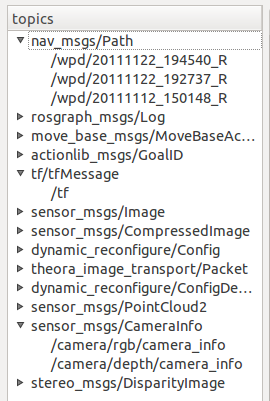
\includegraphics{./graphics/screenshottopics}}
  \end{center}
  \caption{Topic Übersicht}
  \label{fig:topics}
\end{figure}

Die Platzaufteilung zwischen der Topic Übersicht und des Plug-in Tab-Fensters,
innerhalb des Hauptfensters, wurde zugunsten des Plug-in Tab-Fensters gewählt,
sodass dieses mehr Platz einnimmt.  Dies hat zur Folge, dass beim Vergrößern
des Hauptfensters die Fläche des Plus-in Tab-Fensters vertikal und horizontal
vergrößert wird. Die eingenommene Fläche der Topic Übersicht wächst allerdings
nur vertikal wesentlich an. Diese Designentscheidung begründet sich darin,
dass die Plug-ins den wesentlichen Inhalt für den Nutzer präsentieren. Die
Topic Übersicht wird hingegen vermutlich nur kurzzeitig betrachtet werden und
liegt nicht im Zentrum des Interesses. Darüber hinaus ist die Topic Übersicht
sehr kompakt gestaltet und der horizontale Platzbedarf fällt gering aus.


\subsection{Anbindung an ROS}

Die Hauptaufgabe des Rahmens ist es eine Anbindung an ROS zu gewährleisten.
Diese Anbindung muss es den Plug-ins ermöglichen, benötigte Topics zu
abonnieren. Für diese Anbindung ist in Pathcompare die Klasse
\textit{ROSManager} verantwortlich. Im Konstruktor dieser Klasse wird durch
entsprechende ROS API Aufrufe der Node \textit{pathcompare}
erstellt. Dies geschieht durch starten eines separaten Threads, da der ROS Code
in einer eigenen Endlosschleife ausgeführt werden muss, die über die gesamte
Lebenszeit des Nodes bearbeitet wird. Innerhalb dieser Schleife wird
beispielsweise das Eintreffen neuer Messages von abonnierten
Topics abgearbeitet.
Zugriff der Plug-ins auf ROS spezifische Funktionalität wird komplett über den
\textit{ROSManager} gekapselt. Diese Zentralisierung ist nötig, um den Zugriff
der verschiedenen Plug-ins auf ROS zu koordinieren. 
Die zentrale Methode \textit{subscribeToTopic()}, die durch den ROSManager
allen Plug-ins zur Verfügung steht, ermöglicht es eine 
Topic zu abonnieren. Die zu abonnierende Topic wird dabei anhand ihrer
Topic-id identifiziert.


Beim Abonnieren einer Topic wird in ROS typischerweise direkt eine
Methode als Callback angegeben, welche eingehende Messages bearbeitet.
Beim einfachen Abonnieren ist es dabei zunächst nicht möglich, mehrere
Callbacks zu registrieren. Beim einfachen Abonnieren muss außerdem der Message
In Pathcompare bestehen in dieser Hinsicht allerdings zwei
Schwierigkeiten, denen bei der Entwicklung begegnet werden musste:

\begin{enumerate}
  \item eventuell abonnieren mehrere Plug-ins eine Topic
  \item Topics können verschiedene Message Typen haben
\end{enumerate}

Das erste Problem wurde durch die Verwendung von
\textit{ros::message\_filter::cache} gelöst. Objekten dieser Klasse wird bei der
Initialisierung eine Topic zugewiesen. Empfangene Messages
dieser Topic werden in einem Ringpuffer mit einstellbarer Größe
zwischengespeichert.  Außerdem erlaubt diese Klasse die Registrierung beliebig
vieler Callbacks.  Der \textit{ROSManager} sorgt dafür, dass für jede von
den Plug-ins benötigte Topic genau ein
\textit{ros::message\_filter::cache} Objekt existiert. Plug-ins erhalten dann
einen Verweis auf dieses Objekt und können ihren Callback registrieren.
\autoref{fig:rosmanager} ist ein Beispiel für eine Ausführung von Pathcompare
in Verbindung mit drei Plug-ins. Über das ROS werden die drei Topics topic\_x,
topic\_y und topic\_z angeboten. Durch einen Aufruf von der
\textit{subscribeToTopic()} Methode
des ROSManager soll Plug-in 1 die topic\_x abonnieren. Der ROSManager legt aus
diesem Grund einen ros::message\_filter::cache an und gibt einen Verweis darauf
an das Plug-in 1 zurück.
Plug-in 2 möchte dieselbe Topic abonnieren und erhält ebenfalls einen
Verweis auf denselben Cache. Plug-in 3 verlangt jedoch die topic\_y zu
abonnieren und es erfolgt das anlegen eines neuen ros::message\_filter::caches. 

\begin{figure}[t]
  \begin{center}
    \fbox{
\includegraphics{./graphics/rosmanager}}
  \end{center}
  \caption{Anbindung an ROS durch ROSManager}
  \label{fig:rosmanager}
\end{figure}

Das zweite aufgeführte Problem betrifft die Speicherung der Verweise auf
ros::message\_filter::cache Objekte im \textit{ROSManager}. Diese haben
abhängig vom Message Typen der Topic unterschiedliche generische Typen. Dadurch
kann man sie nicht direkt in einer Liste oder vergleichbaren Datenstruktur
hinterlegen. Das Problem wurde gelöst, indem der ROSManager void Zeiger auf die
unterschiedlichen caches speichert.

Weitere Methoden des ROSManagers erlauben es den Plug-ins, im ROS verfügbare
Topics zu erfragen.
Für eine komplette Methodenübersich sei an dieser Stelle auf die
Klassendefinition \textit{rosmanager.h} im Package pathcompare verwiesen.

Die Klasse ROSManager sorgt außerdem dafür, dass die Topic Übersicht
regelmäßig aufgefrischt wird. Dadurch wird dem Nutzer ersichtlich, wann neue
Topics erscheinen oder nicht mehr verfügbar sind. Da die
ROS \gls{API} keinen Event Service anbietet, um Beobachter zu benachrichtigen
falls sich der Status von Topics ändert, stellt der
\textit{ROSManager} sekündlich eine Anfrage an den Master nach dem
aktuellen Stand der Topics. Dies ist gesteuert über einen QTimer in Verbindung
mit dem Signal-Slot Konzept.

\subsection{Laden von Plug-ins}
Das Einbinden von Plug-ins in den Rahmen steuert die Klasse
\textit{PluginLoader}. Sie sucht dabei in einem Verzeichnis nach möglichen
Plug-in Dateien. Bei dieser Suche werden generell nur Shared Library
Dateien betrachtet. Handelt es sich um eine für Pathcompare gültige
Plug-in Datei, wird das Plug-in geladen under der \textit{PluginLoader} erfragt
den Namen des Plug-ins,
über eine im Plug-in Interface spezifizierte Methode \textit{getName()}.
Anschließend wird im Plug-in Tab Fenster ein neuer Tab angelegt. Dabei wird im
Tab Reiter der erfragte Name des Plug-ins eingetragen. Dadurch sind in der GUI
die Plug-ins für den Nutzer leicht zu unterscheiden und können schnell
angewählt werden.  Der Plug-in Ordner steht während der Laufzeit von
Pathcompare unter der Beobachtung des \textit{PluginLoaders}.  Obwohl
Pathcompare bereits gestartet wurde, können also Plug-ins in das
Plug-in Verzeichnis eingefügt werden und diese werden geladen. Dies bietet mehr
Flexibilität für den Nutzer und Entwickler, da kein Neustart der Rahmen
Anwendung sowie der ausgeführten Plug-ins erforderlich ist.

\subsection{Main Compare Plug-in}
\label{sub:maincompare}


\textit{Main Compare} implementiert die eigentliche Hauptfunktionalität, um Pfaddaten des
Referenzsystems und der Sensorknoten zu vergleichen und auszuwerten. 
Es ist dabei der Philosophie von Pathcompare folgend als Plug-in
implementiert worden, welches beim Starten des Rahmens durch den
\textit{PluginLoader} geladen und ausgeführt wird.

In der GUI von Main Compare werden dem Nutzer verschiedene Informationen sowie
Einstellungsoptionen bezüglich der
empfangenen Pfaddaten angezeigt. Die Funktionen der einzelnen GUI Elemente
werden im Folgenden aufgezeigt.
Insgesamt gibt es drei Bereiche in der GUI. Die GUI ist in
\autoref{fig:pathcompare} gezeigt. Die drei Bereiche lassen sich anhand drei
verschiedener Labels abgrenzen. Von oben nach untern gesehen sind
dies die Bereiche:

\begin{enumerate}
  \item Reference path selection
  \item Export results
  \item Results
\end{enumerate}


Der Bereich der ``Reference path selection'' beinhaltet eine Combobox, welche
alle über ROS verfügbaren Topics des Message Typs \textit{nav\_msgs/Path} beinhaltet.
Der Nutzer kann dann aus dieser Liste einen Pfad auswählen, der als
Referenzpfad genutzt werden soll. Das bedeutet, dass der ausgewählte Pfad als
Referenz für die übrigen Pfade gilt. So werden dann die Abstandsberechnungen
bezüglich dieses Pfades durchgeführt. Die Auswahl des Referenzpfades kann
jederzeit geändert werden und die Abstände werden stets neu berechnet.

Unterhalb des ``Reference path selection'' befindet sich der ``Export
results'' Bereich. Er dient dem Nutzer dazu, die berechneten und
im ``Results'' Bereich visualisierten Ergebnisse, permanent zu speichern.
Die Speicherung erfolgt dabei als \gls{CSV} Datei. Der Export wird
durchgeführt, wenn der Nutzer den in diesem Bereich vorhandenen Button drückt. 
Die CSV Datei wird im Ausführungsverzeichnis von Pathcompare abgespeichert.

Für jeden Punkt einer Path Topic wird in der CSV Datei eine Zeile, nach dem in
\autoref{lst:export} gezeigten Format, erstell:

\begin{lstlisting}[caption=Format der Export CSV Datei, label=lst:export]
Topicid;Pfadlaenge;Medianabstand;Varianz;Standardabweichung;Mittelwert;Zeitstempel;x;y;z;Abstand
\end{lstlisting}

Das Trennzeichen für die einzelnen Daten ist das ; Zeichen.


Der ``Results'' Bereich dient dazu, alle ermittelten Informationen bezüglich der
Pfade für den Nutzer anzuzeigen. Die Visualisierung erfolgt hierbei durch eine
Tabellenstruktur. In dieser Tabelle wird für jede Path Topic ein Spalte
angelegt.
In jeder Zeile einer Spalte sind dabei die unterschiedlichen
Informationen eingetragen.
Main Compare verhält sich so, dass Topics, welche einmal in
der Tabelle erfasst wurden, dort verbleiben. Sollte also eine Topic nicht
mehr im ROS zur Verfügung stehen, bleiben die angezeigten Informationen auf
Basis der zuletzt empfangenen Werte dennoch erhalten. 

In der Tabelle werden für den Nutzer folgende Informationen angezeigt:

\begin{itemize}
  \item Anzahl der Lokalisierungen
  \item Berechnung der Pfadlänge
  \item Anzeige des Medians der Abstände
  \item Anzeige des arithmetischen Mittels der Abstände
  \item Berechnung der empirischen Varianz $s^2$ der Abstände
  \item Berechnung der empirischen Standardabweichung $s$ der Abstände
  \item 20 größten Abstände zum Referenzpfad
\end{itemize}

Die angezeigten Informationen werden beim Empfang neuer Pfad Messages stets
aktualisiert. Generell gilt dabei, dass jede Path Message den bisher
zurückgelegten Pfad vollständig
enthalten muss. Pfade können also nicht stückweise übertragen werden. Dieses vorgehen
bietet die Möglichkeit, dass Pfaddaten nachträglich geändert werden können.
Also kann beispielsweise die erste Lokalisierung innerhalb eines Pfades zu einem
späteren Zeitpunkt abgeändert werden. 

Um nachzuvollziehen wie die in Main Compare angezeigten Informationen ermittelt werden, bietet
es sich an, zunächst den Typ der Messages, welche über die Pfad Topics
empfangen werden, zu analysieren. 
Wie bereits beschrieben sind die Messages vom Typ
\textit{nav\_msgs/Path}, der wie folgt definiert ist:

\begin{lstlisting}[caption=ROS Path Message, label=lst:pathmsgs]
Header header
  uint32 seq
  time stamp
  string frame_id
geometry_msgs/PoseStamped[] poses
  Header header
    uint32 seq
    time stamp
    string frame_id
  geometry_msgs/Pose pose
    geometry_msgs/Point position
      float64 x
      float64 y
      float64 z
    geometry_msgs/Quaternion orientation
      float64 x
      float64 y
      float64 z
      float64 w
\end{lstlisting}

Zunächst ist in \autoref{lst:pathmsgs} zu erkennen, dass sich dieser Message Typ aus anderen Typen
zusammensetzt. Auf der obersten Ebene ist dies ein
\textit{Header} und ein Array von \textit{geometry\_msgs/PoseStamped}.
Der Header dient dazu, die Path Message von anderen empfangenen
Path Messages zu unterscheiden und dazu die Messages ordnen zu können. Die Ordnung kann dabei über eine Sequenznummer
(seq) oder einen Zeitstempel (stamp) hergestellt werden. Das Feld
\textit{frame\_id}
definiert einen Bezugsrahmen innerhalb von ROS. Es wird aber im Kontext von
Main Compare nicht ausgewertet und wird hier deswegen nicht genauer erläutert.
Die eigentlichen Pfaddaten verbergen sich in dem Array von PoseStamped. Auch
PoseStamped ist ein zusammengesetzter Typ, bestehend aus einem Header und einer
Pose. Die Pose setzt sich aus einem Point und einer Quaternion zusammen.
Der gefahrene Pfad wird nun dadurch in der Path Message abgebildet, indem bei
jeder durchgeführten Lokalisierung eine PoseStamped angelegt wird. Diese PoseStamped
hält im Header die Zeit der Lokalisierung und eine Sequenznummer fest. In der
Pose wird dann der bei der Lokalisierung ermittelte Ort als Point eingetragen. Die Quaternion
hält fest, welche Ausrichtung dabei im Raum vorliegt und wird auch
in die Pose eingefügt. Die Ausrichtung ist
allerdings optional und wird in der derzeitigen Version von Main Compare nicht beachtet. 

Außerdem lässt sich in \autoref{lst:pathmsgs} erkennen, dass die
Lokalisierungen dreidimensional erfolgen können. Die von Main Compare
ausgeführten Berechnungen sind aber auch mit Daten niederer Dimension möglich,
indem die nicht genutzte Dimension auf 0 gesetzt wird. Beispielsweise werden,
in der derzeitigen Form des Referenzsystems, vom Roboter zweidimensionale
Lokalisierungsdaten in der x-y Ebene übermittelt und die z Komponente erhält
immer den Wert 0. Wie schon in Bezug auf die orientation erwähnt, werden nicht alle Komponenten der
Pfad Message in Main Compare verwendet. Für die derzeitige Version sind
folgende Felder relevant:

\begin{itemize}
  \item poses.stamp (Typ ros::time)
  \item pose.position.x (Typ float64)
  \item pose.position.y (Typ float64)
  \item pose.position.z (Typ float64)
\end{itemize}

Obwohl nicht alle Felder der Path Message genutzt werden, ist dieser Message Typ
für Main Compare die geeignete Wahl, da er in ROS standardmäßig
definiert ist. Dies erspart die Definition und Verteilung eines
eigenen Message Typs. Außerdem sind die ungenutzten Felder nicht
übermäßig groß und werden die Kapazitäten des Übertragungskanals kaum belasten.
Vernachlässigt man die ungenutzten Felder des Header, der eine in ROS definierte Standardmessage ist, fallen nur
zusätzliche 24 Byte für die ungenutzte orientation pro übertragenem Point an.
darüber hinaus ist es denkbar, dass die orientation in späteren Versionen von
Main Compare doch noch betrachtet wird und somit die durchzuführenden
Änderungen klein ausfallen.

Anhand der oben aufgezählten, genutzten Felder lässt sich ein Pfad abstrakt durch eine Menge
$M$ von Tupeln modellieren. Dabei setzen sich die Tupel aus einem Zeitstempel und einem dreidimensionalem
Punkt zusammen. In Anlehnung an die verwendeten Bezeichner in
\autoref{lst:pathmsgs}, sei $M$ demnach wie folgt definiert:

\begin{equation*}
  \label{eqn:setdef}
  M := \{ (p.stamp , p.position) \mid p \in poses \}
\end{equation*}

Die konkrete Repräsentation dieses Modells erfolgt in Main Compare durch die
Klassen \textit{TopicPath} und \textit{Position}. TopicPath repräsentiert dabei
die Menge $M$. Position repräsentiert ein einzelnes Tupel und enthält somit den
Zeitstempel und zugehörigen Punkt. Dem Modell entsprechend enthält ein
TopicPath Objekt eine Liste von Position Objekten.  Neben den Klassen TopicPath
und Position gibt es noch eine Klasse \textit{TopicPathManager}. Es wird genau
ein Objekt dieser Klasse für jede im ROS verfügbare topic mit dem Message Typ
nav\_msgs/Path angelegt. Diese
Klasse bietet eine callback Methode, welche beim zum topic gehörenden
message\_filter::cache registriert wird. Kommt eine neue Message an, wird die
callback Methode aufgerufen und aus den Werten der Path Message ein neues
TopicPath Objekt erstellt. Anschließend werden anhand des neuen TopicPaths
alle nötigen Berechnungen erneut durchgeführt und die Results Tabelle
aktualisiert. Die Beziehung der Klassen Position, TopicPath und
TopicPathManager werden in \autoref{fig:topicpathrelated} verdeutlicht.

\begin{figure}[t]
  \begin{center}
    \fbox{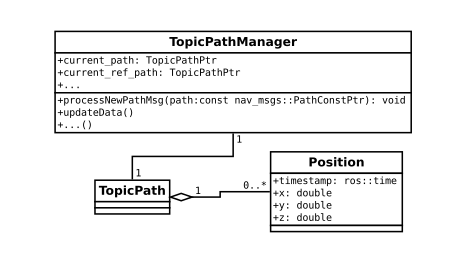
\includegraphics{./graphics/topicpathrelated}}
  \end{center}
  \caption{In Main Compare verwendete Klassen zum verarbeiten von Pfaden}
  \label{fig:topicpathrelated}
\end{figure}

Anhand der abstrakten Modellierung $M$ eines Pfades, werden im Folgenden, die von
Main Compare ausgeführten Berechnungen erläutert. In der konkreten
Repräsentation erfolgen alle Berechnungen in der Klasse \textit{TopicPathManager}. 

\subsubsection{Anzahl der Lokalisierungen}
Um die Anzahl der Lokalisierungen zu ermitteln, wird in Main Compare lediglich die
Mächtigkeit der Menge $M$ bestimmt. Es gilt also:

\begin{equation*}
  \label{eqn:numofpoints}
  number of points = \vert M \vert
\end{equation*}

Im \textit{TopicPathManager} ist dies entsprechend einfach realisiert.

\subsubsection{Berechnung der Pfadlänge}
Bei der Bestimmung der Pfadlänge werden zunächst alle Abstände zwischen je
zwei direkt aufeinanderfolgenden Punkten im Pfad bestimmt. Die Summe all dieser
Abstände entspricht dann der Gesamtlänge des Pfades. Dazu muss jedoch noch
geklärt werden, wann ein Punkt $p_2$ in einer Path Message auf einen anderen
Punkt $p_1$ folgt. Das lässt sich über den Zeitstempel feststellen und ist
anschaulich ausgedrückt dann der Fall, wenn keine weitere Lokalisierung in
der Zeit zwischen den Lokalisierungen $p_1$ und $p_2$ stattgefunden hat. Dies
kann man abstrakt und bezogen auf $M$ ausdrücken.  Ein Punkt $p_2$ ist direkt
folgend auf einen Punkt $p_1$, genau dann wenn für die zugehörigen Tupel

$t_1 := (z_1, p_1)$ und $t_2 := (z_2, p_2)$
mit
$t_1,t_2 \in M$
gilt, dass:
\[
z_2 > z_1 \wedge \nexists (z^{,}, p^{,}) \in M : z_2 > z^{,} > z_1
\]

Der Abstand zweier aufeinanderfolgender Punkte lässt sich einfach durch
Vektorsubtraktion und anschließende Betragsbildung des resultierenden Vektors
bestimmen.

\subsubsection{Pfadvergleichsverfahren und Abstandsberechnung}

Das Hauptziel von Main Compare ist es, dem Nutzer zu erleichtern, die
Genauigkeit eines durch Lokalisierung gewonnenen Pfades, in Bezug auf einen
Referenzpfad, abzuschätzen. Um dies zu tun, ist es notwendig, den Abstand von
Lokalisierungen des zu untersuchenden Pfads, zu denen des Referenzpfads, zu
ermitteln. In einem naiven Ansatz kann man die Lokalisierungen direkt
miteinander vergleichen. Voraussetzung hierfür ist, dass für jeden Punkt des Referenzpfades auch
ein Punkt im zu vergleichenden Pfad mit demselben Zeitstempel existiert. Der
Vergleich zwischen Referenz- und zu untersuchendem Pfad fällt dann denkbar
einfach aus, denn man muss nur den Abstand je
zweier Punkte, mit demselben Zeitstempel, bestimmen.
Das Problem bei dieser Methode ist jedoch, dass das Referenzsystem und die
einzelnen Sensorknoten unabhängig voneinander sind und dadurch Lokalisierungen
nicht immer zum selben Zeitpunkt oder mit einer anderen Frequenz durchführen 
können. Um dies zu verhindern, müsste man einen zentralen
Taktgeber in das System integrieren, der durch ausgesendete Impulse, zum
Beispiel in der Form einer ROS Message, den Komponenten vorschreibt,
wann eine Lokalisierung durchgeführt werden soll.
Die Einführung eines solchen Taktgebers verkompliziert jedoch die
Testausführung und setzt bei allen am Test beteiligten Komponenten voraus, dass
deren Software auf diesen Mechanismus reagiert. Zudem ist man während des Tests
zwingend auf eine ungestörte Netzwerkkommunikation angewiesen, da sonst der
Impuls nicht zeitgleich oder gar nicht bei den Komponenten ankommt.

Aufgrund dieser schwerwiegenden Nachteile wurde bei der Entwicklung von Main
Compare ein Ansatz gewählt, der es den Komponenten erlaubt Lokalisierungen zu
beliebigen Zeitpunkten und mit beliebiger Frequenz durchzuführen. Die einzige
Voraussetzung ist dabei, dass die Uhren der Komponenten, mit einem gewissen
tolerierbaren Fehler, synchronisiert werden. Dies sichert, dass die Zeitstempel der
Lokalisierungen zuverlässig vergleichbar sind. Der Abstand wird wie folgt
ermittelt. Der Prozess der Abstandsbestimmung ist auch
\autoref{fig:distancetoref} dargestellt.


\begin{figure}[t]
  \begin{center}
    \fbox{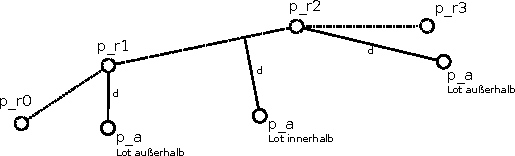
\includegraphics{./graphics/distancetoref}}
  \end{center}
  \caption{Bestimmung der Distanz eines Punktes $p_a$ zum Referenzpfad}
  \label{fig:distancetoref}
\end{figure}

Für jeden Punkt im zu vergleichenden Pfad $A$
wird der Abstand zum Referenzpfad $R$ bestimmt. Dazu wird der jeweilige
Zeitstempel $z_a$ eines Punktes $p_a$ aus A einem passenden
Zeitstempelintervall zweier aufeinanderfolgender Punkte $p_{r2}$ , $p_{r1}$ aus $R$ zugeordnet, sodass
gilt:

\[
z_{r1} <= z_a < z_{r2}
\]

Ist dieses Intervall gefunden, wird der Abstand von $p_a$ zum Geradensegment
$\overline{p_{r2} p_{r1}}$ bestimmt. Um diesen Abstand zu bestimmen, wird das
Lot auf die von $p_{r1}$ und $p_{r2}$ bestimmte Gerade ermittelt. Fällt das Lot
dabei zwischen $p_{r1}$ und $p_{r2}$ auf die Gerade, wird der Abstand vom
Lotpunkt zu $p_a$ errechnet. Fällt er jedoch außerhalb dieses Intervalls, muss
der Abstand, je nach Lage des Lotpunkts, entweder zu $p_{r1}$ oder $p_{r2}$
bestimmt werden. 

Charakteristisch bei dieser Art der Abstandsbestimmung ist, dass beim
Referenzpfad zwischen zwei Lokalisierungen die ausgeführte Bewegung durch eine
Gerade interpoliert wird. 
Es wird also angenommen, dass die tatsächlich
ausgeführte Bewegung zwischen den Punkten einer Gerade entspricht. Daraus
folgt aber, dass man die Lokalisierungsfrequenz des Referenzpfades an die
Bewegungsgeschwindigkeit des Roboters anpassen muss. Dabei soll
zwischen zwei Lokalisierungen des Referenzpfades die interpolierte Strecke
klein bleiben, denn dadurch nähert sie sich stärker der tatsächlich gefahrenen
Strecke an. Betrachtet man das derzeitige Referenzsystem mit dem TurtleBot, so
ist die Bewegungsgeschwindigkeit allerdings gering und eine sekündliche
Lokalisierung erscheint ausreichend. Dies muss jedoch noch durch weitergehende
Tests bestätigt werden.

%TODO evtl. Verweis auf TopicPathManager::   Methode

\subsubsection{Bestimmung empirischer Varianz und Standardabweichung}
Auf Basis der zuvor beschriebenen Abstandsberechnung wird in Main Compare die
empirische Varianz der Abstände bestimmt. Um diese zu berechnen, wird zunächst
das arithmetische Mittel gebildet, welches ebenso in der Results Tabelle angezeigt wird.
Anschließend wird die empirische Varianz $s^2$ gebildet. Die empirische Standardabweichung
ist die Wurzel aus $s^2$ also $s$.

\subsubsection{Bestimmung des Median der Abstände}
Der Median der Abstände ist robuster gegenüber Ausreißern als das
arithmetische Mittel und wird deshalb zusätzlich der Results Tabelle
aufgeführt.

\subsection{Das Plug-in Konzept}

Im folgenden Abschnitt wird das Konzept des Pathcompare Plug-in Mechanismus
erläutert und aufgezeigt welche Schritte erforderlich sind, um eigene Plug-ins
für Pathcompare zu erstellen. Realisiert sind die Plug-ins in Pathcompare
mithilfe der Qt Plug-in API. Diese gibt Strukturen vor, um Plug-ins zu
definieren. Außerdem beinhaltet sie Klassen, um Plug-ins während der Laufzeit
einer Applikation zu laden.  Zum Erstellen von Plug-ins mithilfe dieser API
müssen im wesentlichen zwei Schritte ausgeführt werden:

\begin{enumerate}
  \item Definition eines Interfaces
  \item Implementierung des Interfaces durch Plug-in
\end{enumerate}

Das Interface legt fest, welche
Methoden durch ein Plug-in zu implementieren sind. Das Interface hat dabei die
Form einer Klassendefinition mit nur rein virtuellen Funktionen. Zusätzlich
wird diese Klassendefinition durch Qt Makros ergänzt, um es als Interface zu
markieren. In Pathcompare ist dieses Interface vorgegeben und trägt den Namen
\textit{ComparatorPluginFactoryInterface}. Wie die Implementierung dieses
Interfaces erfolgt, wird nun anhand eines vorhandenen Plug-ins für Pathcompare
erläutert. Dieses Plug-in trägt den Namen Camera View. In der derzeitigen
Version von Pathcompare wird es, ebenso wie Main Compare, beim Starten der
Anwendung geladen. Es dient dem Nutzer dazu ROS Topics des Message Typs
\textit{sensor\_msgs/Image} zu visualisieren. Dieser Message Typ wird
beispielsweise innerhalb von ROS genutzt, um Kamerabilder der Kinect zur
Verfügung zu stellen.  Camera View könnte also bei einer Fahrt des TurtleBots
eingesetzt werden um dem Tester ein Bild der aktuellen Umgebung des Roboters zu
vermitteln. Die Gestaltung der Camera View GUI ist in \autoref{fig:cameraview}
gezeigt.  Der Nutzer kann mit einer Combobox eine Topic des Typs
sensor\_msgs/Image auswählen. Nach der Auswahl werden die empfangenden Bilder
der gewählten Image Topic eingeblendet. 

\begin{figure}[t]
  \begin{center}
    \fbox{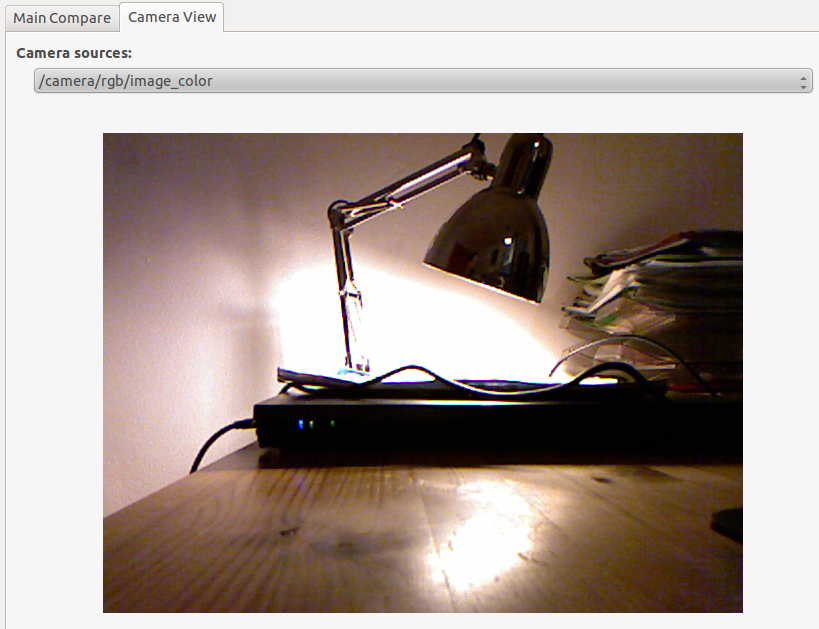
\includegraphics{./graphics/screenshotcameraview}}
  \end{center}
  \caption{GUI des Camera View Plug-ins}
  \label{fig:cameraview}
\end{figure}

Wie zuvor beschrieben, muss jedes Pathcompare Plug-in das Interface
\textit{ComparatorPluginFactoryInterface} implementieren, so auch Camera View.

Dieses Interface beinhaltet die zwei in \autoref{lst:factoryinterface}
gezeigten Methoden.

\begin{lstlisting}[caption=Interfacemethoden - Plug-ins müssen diese implementieren , language=C++, basicstyle=\footnotesize, label=lst:factoryinterface]

        virtual ComparatorPluginPtr createComperatorPlugin(ROSManager * ros_manager, QWidget *tab_widget) const = 0;
        virtual QString getPluginName() const = 0;

\end{lstlisting}

Die Methode createComparatorPlugin() ist eine Factorymethode und erzeugt das
eigentliche Objekt, welches die Funktionalität des Plug-ins beinhaltet. Dieser
Umweg ist notwendig, da Qt Plug-ins keine typischen Objekte sondern
shared libraries sind. In einer shared library können
zwar Methoden ausführbar hinterlegt werden, aber kein eigenständiges Objekte
mit Attributen existieren. Der Rückgabetyp von createComparatorPlugin() ist
ComparatorPluginPtr, definiert durch \autoref{lst:returntypedef}.

\begin{lstlisting}[caption=Typdefinition von CompoaratorPluginPtr, language=C++, basicstyle=\footnotesize, label=lst:returntypedef]
//typedef for shared_ptr reference to ComparatorPlugin
typedef boost::shared_ptr<ComparatorPlugin> ComparatorPluginPtr;
\end{lstlisting}

Es handelt sich also um einen Verweis auf ein Objekt der Klasse
ComparatorPlugin. Diese Klasse ist der Basistyp, für das in der Factory Methode
dynamisch erzeugte Objekt. In Camera View ist die createComparatorPlugin()
Factory Methode wie folgt implementiert worden, siehe \autoref{lst:create}:

 \begin{figure}[t]
   \begin{center}
     \fbox{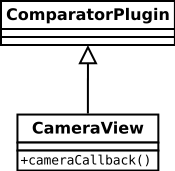
\includegraphics{./graphics/cameraviewcomparator}}
   \end{center}
   \caption{ComparatorPlugin als Basisklasse zu CameraView}
   \label{fig:cameraviewcomparator}
 \end{figure}

\begin{lstlisting}[caption=Implementierung der createComparatorPlugin in Camera View, language=C++, basicstyle=\footnotesize, label=lst:create]
ComparatorPluginPtr PathcompareMainFactoryPlugin::createComparatorPlugin(ROSManager * ros_manager, QWidget *tab_widget) const
{
        ComparatorPluginPtr comp_plugin(static_cast<ComparatorPlugin *>(new CameraView(ros_manager, tab_widget)));
        return comp_plugin;
}
\end{lstlisting}

Es wird hier ein Objekt des Typs CameraView angelegt. Dieses
hat wie in \autoref{fig:cameraviewcomparator} gezeigt den Basistyp ComparatorPlugin. Im
Konstruktor erhält es Verweise auf den ROSManager, welcher benötigt wird um ROS
spezifische Aktionen durchzuführen. Als zweites Konstruktorargument wird die
Zeichenfläche für die Camera View GUI übergeben. Am Ende der Methode wird das
fertig angelegte Objekt zurückgegeben und steht damit Pathcompare als Plug-in zur
Verfügung. 

Die zweite Methode im Plug-in Interface, getName() liefert lediglich den Namen
des Plug-ins zurück und wird in Pathcompare durch die Klasse PluginLoader
genutzt.

Zusammenfassend kann man sagen, dass die eigentlichen Pathcompare Plug-in Interface
Methoden ohne großen Aufwand zu implementieren sind. Ein vollständiges
Beispiel zur Implementierung neuer Plug-ins ist durch Camera View gegeben.
Zu finden sind dabei alle relevanten Code- und Builddateien im Package 
\textit{pathcompareplugins/cameraview}

